\section{Konzept}\label{sec:konzept}
Das folgende Kapitel soll Gedanken zur Realisierung des Projekts widerspiegeln. 
Dies umfasst den allgemeinen Systemaufbau, sowie Entwürfe und Architekturvorstellungen hinsichtlich der Server- und Clientseite und die damit verbunden eingesetzten Softwaremodule.
\subsection{Systemaufbau}\label{sec:sysaufbau}
Das System soll in eine Server- und Clientseite aufgeteilt sein. 
Da es sich um eine Webapplikation handeln soll, wird die Interaktion mit dem Server über einen Webbrowser stattfinden und dieser soll auch gleichzeitig der Client sein. Für eventuelle Wartungsaufgaben und Aufgaben wie das Starten des Servers, soll die Steuerung über eine Kommandozeile möglich sein. Alle anderen Interaktionen werden über den Client ausgeführt.
\subsection{Netzwerkaufbau}\label{sec:netzwerkaufbau}
Als Kommunikationsprotokoll soll das aus dem Webbereich bekannte HTTP resp. HTTPS Protokoll zum Einsatz kommen. Der Server wird als Webserver fungieren, Anfragen müssen vom Client aus initiiert werden (vgl. Abschnitt \ref{sec:www}). Bei Parts, welche Echtzeitinteraktion benötigen, soll das Websocket (ws) Protokoll zum Einsatz kommen, welches eine bidirektionale Kommunikation zwischen Server und Client ermöglicht. Der Server soll sowohl in einem Intranet wie auch im Internet lauffähig sein. Dabei kann er, je nach infrastruktureller Realisierung über ein IPv4 oder IPv6 Adresse erreicht werden, bei Nutzung eines DNS-Servers auch über eine Domain.\\ \\
Schlussfolgernd aus Systemaufbau und Netzwerkaufbau lässt sich folgende Abbildung skizzieren:

\begin{figure}[H]
	\centering
	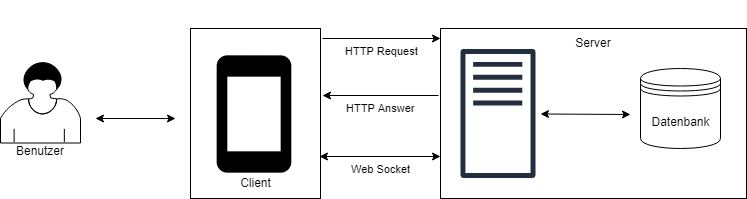
\includegraphics[width=0.8\linewidth]{bilder/server_diagram}
	\caption[Kommunikationsaufbau des zu entwickelnden Systems]{Kommunikationsaufbau des zu entwickelnden Systems}
	\label{fig:server_diagram}
\end{figure}


\subsection{Entwurf des Servers}\label{sec:serverkonzept}
Aufbauend auf das Grundlagen und Analysekapitel sollen in diesem Abschnitt die Entwurfsgedanken hinsichtlich der Serverkomponente des Projekts widergespiegelt werden. 
\subsubsection{Laufzeitumgebung: Node.js}\label{sec:nodejs}
Als Laufzeitumgebung und Grundbaustein des Servers soll die JavaScript-Laufzeitumgebung Node.js genutzt werden, da dies zwei wesentliche Vorteile mit sich bringt:
\begin{enumerate}
	\item Node.js nutzt als Paketmanager und Projektverwaltungstool \textbf{NPM} (Node Paket Manager). Mit dieser Software ist der Zugang zu über 350.000 Paketmodulen (Stand 13. Januar 2017) gegeben und diese können das Projekt Modular erweitern. Ebenso können mit NPM grundlegende Start- und Installationsskripte leicht ausgeführt werden. 
	\item Da Node.js eine JavaScript-Laufzeitumgebung ist, wird zur Programmierung die Skriptsprache JavaScript genutzt, welche auch auf der Clientseite im Webbrowser zum Einsatz kommt. Dies erleichtert den Implementierungsprozess, da einheitlich in einer Sprache geschrieben wird.
\end{enumerate}
Darüber hinaus können NPM-Pakete auch auf der Clientseite genutzt werden (siehe dazu auch Abschnitt \ref{sec:browserify}). Eine gute Skalierbarkeit ist ebenfalls gegeben. Dies wird in folgenden Abschnitten genauer erläutert. Ist ein besonders hohen Ressourcenbedarf von Nöten (z.B. eine Bildungseinrichtung möchte einen zentralen Server installieren, welche viele Klassen/Kurse bedienen soll) können mehrere Serverinstanzen auf einer Maschine parallel laufen und vorab mit einem Lastenverteiler (Load Balancer) Server, wie z.B. NGINX verwaltet werden. Durch die genannte Argumentation soll das Projekt mit NodeJS realisiert werden und nicht mit einem php-Framework. \\ Da Node.js grundlegend sehr offen ist was seinen Einsatzzweck betrifft, soll als Webserver Modul das Node-Paket \textbf{Express.js} genutzt werden, welches im nächsten Abschnitt genauer erläutert wird.
\subsubsection{Webserver: Express}\label{sec:expressjs}
Um mit Node.js komfortabel eine Webapplikation zu implementieren, soll das bekannte Web-Framework Express eingesetzt werden, welches viele HTTP-Dienstprogrammmethoden und den Einsatz von Middlerwarefunktionen gestattet. Hierbei wird jeder eingehende HTTP Request von Funktion zu Funktion weitergeleitet (Aufruf der Methode \texttt{next()}) oder explizit beantwortet (Die Funktion besitzt ein Rückgabewert). Ebenso ist mit Express das Abbilden von Routen möglich. Express soll für den gesamten administrative Teil des Lehrer-Login zum Einsatz kommen. Ebenso soll durch Express das Anlegen und Editieren von Lehreinheiten möglich sein (vgl. \ref{sec:sysbeschreib}). 
Da für den gesamten Lehrer-Backendbereich Express zum Einsatz kommen soll und hier mit einfachen HTTP-Requests gearbeitet wird, kann auf der Einsatz von JavaScript auf der Client-Seite auf ein Minimum reduziert werden, was den Einsatz auf Servereinheiten mit nicht modernem Webbrowser entgegenkommt (Sollte Client und Server auf der gleichen Maschine ausgeführt werden).\\ \\ 
Für den interaktiven Part des Projekts sollen zur Kommunikation WebSockets genutzt werden, welche mithilfe der JavaScript-Bibliothek \textbf{Socket.IO} realisiert werden sollen. Dies wird in der nächsten Sektion beschrieben.   

\subsubsection{SocketIO}\label{sec:socketio}
Die JavaScript-Bibliothek Socket.IO ermöglicht bidirektionale Echtzeit-Kommunikation zwischen Webclient und Server, wobei dabei Bibliothek sowohl auf Server- wie auch Clientseite zum Einsatz kommt. Ein großer Vorteil ist, dass beide Komponenten eine nahezu identische API aufweisen. Daten können sehr einfach von Client ereignisgetrieben (event-driven) zwischen Server und Client sowie vice versa ausgetauscht werden. Client und Server lauschen dabei gegenseitig auf Ereignisse, wie das Verbinden eines neuen Clients oder auch selbst implementierte Ereignisse. Dabei können jegliche JavaScript Daten hin-und hergeschickt werden. Eine händische Konvertierung in das JSON-Format ist nicht notwendig. Für das Anmelden von Schülerinnen und Schülern, das Durchführen von interaktiven Unterrichtsmethoden soll SocketIO zum Einsatz kommen. Hierzu soll Express die entsprechenden Client Daten auf einer festgelegten Route senden und anschließend die Kommunikation von SocketIO kontrolliert werden. Da die Nutzung der Software rein im Intranet nutzbar ist und Nutzende über ein WLAN Zugriff erhalten können, ist der im Abschnitt \ref{sec:websockets} genannte Nachteil von erhöhtem Datenverkehr zu vernachlässigen.      
\subsubsection{Sonstige Module}
Neben Express ist der Einsatz von weiteren Modulen (Node Packages) vorgesehen, welche unterschiedliche Funktionalitäten realisieren sollen. Diese sind:
\begin{itemize}
	\item \textbf{Body-Parser}: Diese Modul ermöglicht das einfach Auslesen von HTTP-Requests möglich. Schickt ein Client bspw. Formulardaten können diese einfach gelesen und ausgewertet werden. Dies soll im Backendbereich der Lehrenden oftmals die Praxis sein.
	\item \textbf{express-session}: Da Lehrende und Administratoren zur Nutzung der Software einen gültigen Zugang besitzen müssen, ist zur Authentifizierung des Nutzenden der Einsatz von Sessions vorgesehen (Querverweis Abschnitt\ref{sec:www}). Das Modul Express-Session macht das Arbeiten mit diesen sehr komfortabel. Über das Zusatzmodul \texttt{connect-session-sequelize} ist die Zusammenarbeit mit der gewählten Datenbank einfach. (Weiterführende Informationen diesbezüglich im Abschnitt  \hyperref[sec:datenbank]{Wahl der Datenbank}). 
	\item \textbf{Pug}: Die Template Engine Pug besitzt seine eigene Syntax und macht das Entwerfen und Schreiben von HTML Templates, welche serverseitig übermittelt werden, sehr komfortabel. Zusätzlich werden Funktionalitäten wie Vererbung und Mixins unterstützt. Ein Einsatzbeschreibung erfolgt in Kapitel \hyperref[sec:implementierung]{Implementierung}. Pug soll für sämtliche zu übertragende HTML Dokumente zum Einsatz kommen.   
\end{itemize}
\subsubsection{Wahl der Datenbank}\label{sec:datenbank}
Da bei dem zu entwickelnden System vielerlei Daten anfallen, wie registrierte Nutzer, angelegte Kurse, interaktive Unterrichtseinheiten und mehr, ist der Einsatz eines Datenbanksystems unerlässlich. Grundlegen können Datenbanksysteme in zwei Kategorien unterteilt werden: \\
\textbf{SQL} und \textbf{noSQL} Systeme. \\ SQL Systeme speichern ihren Daten in sogenannten Relationsmodellen, welche als Tabelle visualisiert werden können. Hierbei beschreibt der Tabellenkopf den Datensatz und seine Datentypus (jede Spalte für sich) während Zeilen eine Entität (Eintrag) in der Datenbank beschreiben. Vorteil hierbei ist, dass die Daten konform sind, d.h. bei Zugriff liefert immer einen Rückgabewert \cite{neumann2015entwicklung}. Nachteil ist der erhöhte Aufwand, sollte die Definition des Relationsmodells im Nachhinein geändert werden, was das Aktualisieren sämtlicher Daten erfordern würde. Desweiteren sind SQL System schwer skalierbar, da für größere Datenbanksysteme potentere Server gekauft werden müssen. Mehrere Relationsmodelle können über Fremd-Schlüsse (Querverweise) miteinander verbunden werden, um auch komplexere Sachverhalte abbilden zu können. \\ \\ NoSQL lassen sich in verschiedene Subkategorien je nach Arbeitsweise beim Speichern der Datensätze einteilen\cite{neumann2015entwicklung}. Am populärsten sind Dokumentenorientiert, Key-Value Pairs (Schlüssel-Wert Paare) und Graphen-basierte Systeme. Dokumentenorientierte NoSQL Datenbanken legen pro Entität ein Dokument an, in welchem die Informationen meist im JSON Format abgespeichert werden. Key-Value Systeme verfolgen ein einfaches Zuordnungsprinzip und bilden Schlüssel-Wert Paare, ähnlich einer Dictionary Datenstruktur. Bei Graphen-basierten Systemen werden Entitäten und ihre Beziehungen untereinander an sich gespeichert. Generell sind NoSQL Systeme weniger statisch definiert im Vergleich zu SQL Systemen. Dies räumt eine große Flexibilität beim Speichern von Daten ein, da Datensätze auch unvollständig gespeichert werden müssen. Dies kann auch als Nachteil interpretiert werden, ist aber generell immer vom Kontext des Projekts abhängig. \\ \\    

Für das zu entwickelnde System soll ein möglichst flexibler Weg gewählt werden was die Wahl der Datenbank betrifft. Da das MVC-Prinzip zum Einsatz kommen soll, beschreibt der Modell Teil von zu bereitstellenden Daten auch wie diese über welche Funktionalität aus der Datenbank geladen werden sollen. Den Controller soll nur die vom Modell bereitgestellten Funktionalitäten nutzen und keine direkten Datenbankzugriffe selbst ausführen. Damit die Software im hohem Maße skalierbar bleibt, ist der Einsatz eines sogenannter Object-Relationship-Mapper, kurz ORM, (Objektrelationale Abbildung) vorgesehen, der an verschiedenste Datenbanksysteme angebunden werden kann. Da das Projekt in seiner kleinsten Skalierung lokal auf einem Einplantinencomputer wie dem Raspberry Pi 3 und im lokal im Intranet laufen können soll, ist für den Anfang die Verwendung eines Datenbanksystems, welches vollständig durch eine Programmbibliothek lauffähig ist, vorgesehen. Dies hat den Vorteil, dass kein extern laufendes Datenbanksystem installiert, gewartet und gestartet werden muss, da die komplette Datenbank in einer einzigen Datei auf dem Server gespeichert wird. Diese Anforderungen erfüllt die gemeinfreie Programmbibliothek \textbf{SQLite}. Die gesamte Datenbank kann hier sogar rein im Arbeitsspeicher gehalten werden, was jedoch den Nachteil mit sich bringt, dass bei einem Ausfall oder Abschalten des Server der kompletten Verlust sämtlicher Daten mit einhergeht. 
\\ Als ORM fiel die Wahl auf das Node.js Modul Sequelize, welches neben SQLite mit viele andere bekannte SQL Datenbanksystemen zusammenarbeiten kann, u.A. Postgres, MariaDB und Microsoft SQL Server. Der Wechsel auf ein anderes SQL Datenbanksystem ist somit jederzeit problemlos möglich, falls gewünscht. \\ \\  

Das Zusatzmodule \texttt{connect-session-sequelize} ermöglicht eine einfache Handhabung der Session-Verwaltung von eingeloggten Lehrenden in das System. Dazu werden entsprechende Tabellen zur Verwaltung der Sessions und deren Lebenszeit automatisch in der Datenbank  via Sequelize angelegt. Zuvor sollen die Passwörter sicher gespeichert werden, d.h. nicht im Klar-Text, nur als Hashwerte welche zusätzlich mit einem Salt verstärkt werden\footnote{Weiterführende Informationen unter:  \url{https://de.wikipedia.org/wiki/Salt_(Kryptologie)}}.

Da zum Zeitpunkt der Recherche kein zu SQLite ähnliches und für den produktiven Einsatz bereites NoSQL Äquivalent gefunden werden konnte, fiel die Wahl auf SQLite. Die genannten Vorteile eines NoSQL Systems scheinen für die Anforderungen des zu entwickelenden Systems ohnehin nicht relevant, obgleich sogar ein Umstieg auf NoSQL Datenbkansystem möglich wäre, auch wenn dies mit einem etwas erhöhten Aufwand einhergeht, da dann auch der ORM gewechselt und die Modelle entsprechend angepasst werden müssten.  

\subsubsection{Serverarchitekturdiagramm}\label{sec:serverarchitekt}
Schlussfolgernd lässt sich der finale Entwurf des Servers folgend visualisieren und wird in Kapitel \textbf{\ref{sec:implementierung} Implementierung} umgesetzt.

\begin{figure}[H]
	\centering
	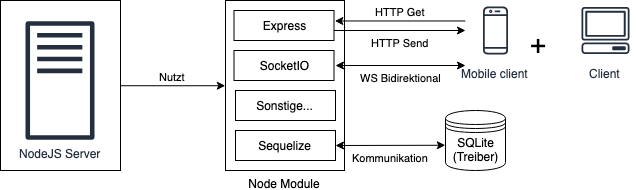
\includegraphics[width=0.8\linewidth]{bilder/server_architektur}
	\caption[Aufbau der geplanten Serverarchitektur]{Aufbau der geplanten Serverarchitektur}
	\label{fig:server_diagram}
\end{figure}
\footnotesize{Hinweis: NodeJS Module aus der Sektion \textbf{Sonstige Module} wurden aus Gründen der Visualisierung in dieser Grafik nicht näher betrachtet. }

\subsection{Entwurf des Clients}\label{sec:clientkonzept}
Wie zuvor erörtert, ist es vorgesehen drei verschiedene Clients zu implementieren, welche alle auf dem gleichen Prototyp basieren sollen, allerdings verschiedene Zwecke verfolgen. Dies sieht ein Webclient jeweils für \textbf{Lehrende/Dozierende}, \textbf{Schülerinnen und Schüler} und einen für \textbf{Großbildanzeigen} optimierten wie Projektoren o.Ä. vor. Zur Vereinfachung werden diese gemäß der vorherigen Reihenfolge \textbf{Teacher Client}, \textbf{Student Client} und \textbf{Presenter Client} in diesem und darauffolgendem Kapitel genannt.\\ \\ 

\subsubsection{Gedanken zu UI}\label{sec:uientwurf}
// TODO am CSS Tag schreiben!
\subsubsection{Browserify}\label{sec:browserify}
Um das Nutzen von Node.js Packages sowie damit verbundene \texttt{require()} Funktionalität auch auf der Clientseite zu ermöglichen, soll die JavaScript Bibliothek \textbf{Browserify} zum Einsatz kommen. Mit ihr können alle Node.js Packages, welche über den Node Package Manager in das Projekt hinzugefügt wurde im Webbrowser des Clients genutzt werden. Dazu bündelt die Bibliothek alle Module und stellt anschließend eine einzige JavaScript Datei zur Verfügung, die nur noch im HTML-Dokument eingebunden werden muss. Mithilfe der \texttt{require()} Funktionalität, welche von Node.js gestellt wird, kann der Code auch übersichtlicher in mehrere Dateien/Module aufgeteilt werden. Dies war ohne Aufwand auf der Browserseite nicht ohne weiteres möglich, ist aber durch die Einführung von Modulen seit ECMAScript\footnote{Der als ECMAScript (ECMA 262) standardisierte Sprachkern von JavaScript beschreibt eine dynamisch typisierte, objektorientierte, aber klassenlose Skriptsprache. (Wikipedia.org)} in Version 6  nun möglich. Oftmals wird aber aus Kompatibliltätsgründen  zu älteren Webbrowsern auf Lösungen wie Browserify oder auch Babel gesetzt. Letztere übersetzt den geschriebenen JavaScript Code so, dass er auch von älteren Webbrowsern interpretiert wird (auch Transpiler genannt). Sämtliche folglich genannten JavaScript Module resp. Bibliotheken sollen via Browserify in eine JavaScript Datei zusammengefasst werden und anschließend pro Client eingebunden werden. Das bringt den zusätzlichen Vorteil dass für jegliches, auf Browserseite eingesetztes JavaScript nur einen einzigen HTTP-Get Request benötigt, da wie erwähnt nur eine JavaScript Datei pro Client angefordert werden muss. 
\subsubsection{JavaScript Lösungen}\label{sec:clientjs}
Von folgenden JavaScript Lösungen soll auf der Clientseite Gebrauch gemacht werden, um den Implementierungsprozess zu optimieren:
\begin{itemize}
	\item \textbf{VueJS}: Um das Anzeige, Editieren und Anpassen dynamischer Inhalte zu erleichtern, soll das JavaScript-Webframework VueJS zum Einsatz kommen, da dieses gut skalierbar ist und alle benötigten Funktionalitäten mit sich bringt. Im Vergleich zu AngularJS und React (siehe auch Abschnitt \ref{sec:clientseitigeransatz}), biete VueJS eine flachere Lernkurve und kann als ein guter Kompromiss aus seinen zwei Konkurrenten betrachtet werden. Mittlerweile hat VueJS seinen Konkurrent React in Sachen Popularität auf GitHub überholt\cite{Daityari2019}. VueJS ist auch gemessen an der Dateigröße von nur 80 KB deutlich kleiner im Vergleich zu Angular mit 500 KB.
	\item \textbf{SocketIO}: Das bereits in Abschnitt \ref{sec:socketio} erwähnte SocketIO besitzt ein Gegenstück, welches auf der Clientseite im Webbrowser zum Einsatz kommt. Dadurch wird die bidirektionale Kommunikation mit der Server ermöglicht und es soll in beide Richtungen Daten in Echtzeit ausgetauscht werden. 
	\item \textbf{Zingchart}: Zur Visualisierung der Wörterwolke (WordCloud), welche bei der interaktiven Unterrichtsmethode Brainstorming zum Einsatz kommt, und sonstigen Diagrammen soll die auf diese Szenarien spezialisierte JavaScript Bibliothek ZingChart genutzt werden. Die Software ist in einer freien Version erhältlich, wobei lediglich ein kleines ZingChart Logo stets angezeigt werden muss\cite{zingchartpricing}.
\end{itemize}

\subsubsection{Lehrer - Bereich}\label{sec:lehrerbereich}
\subsubsection{Schüler - Bereich}\label{sec:schuelerbereich}